\documentclass{article}
\usepackage[pdftex]{hyperref}
\usepackage[pdftex]{graphicx}
\usepackage{fullpage}
\usepackage{color}
\usepackage{hyperref}
\usepackage{wrapfig}
\title{ORC File Format Specification}
\author{Owen O'Malley\\omalley@apache.org}
\date{October 2014}
\begin{document}
\maketitle

\section{Introduction}

\begin{wrapfigure}{r}{3.1in}
  \centering
  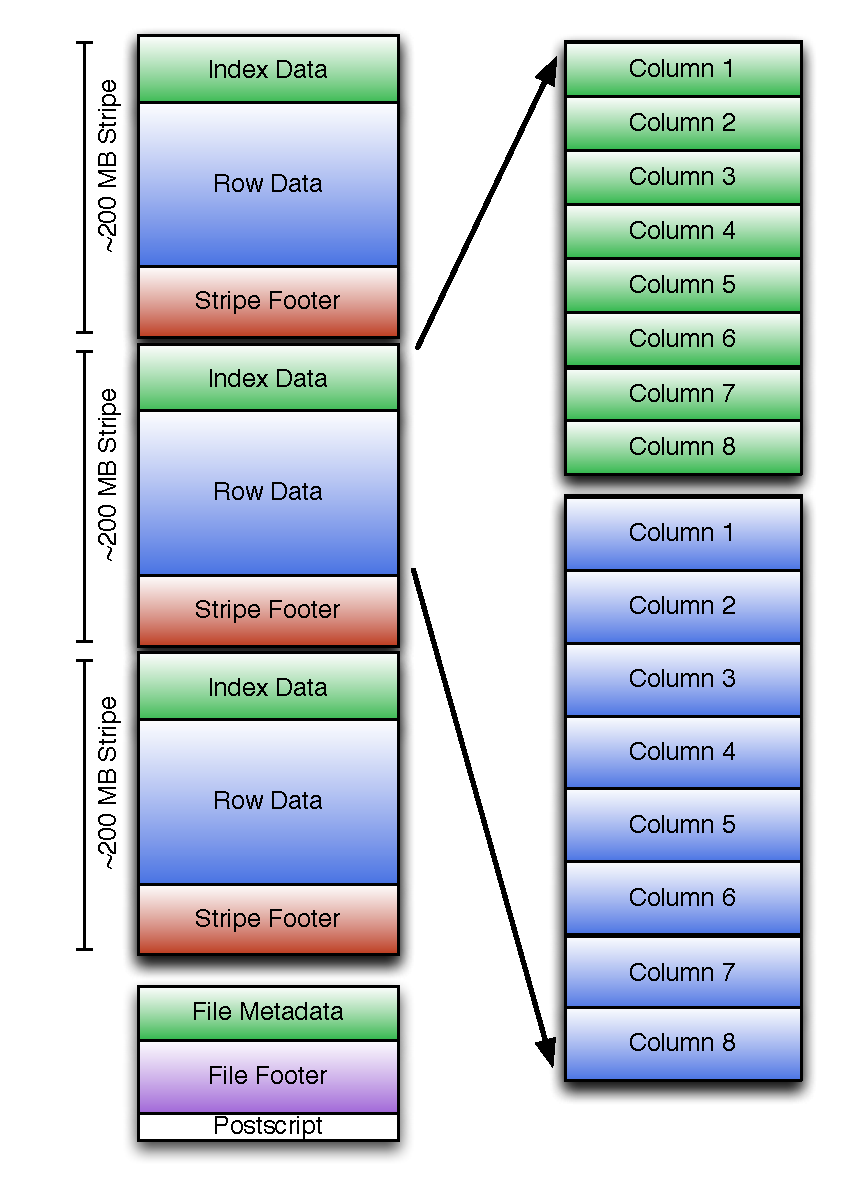
\includegraphics[width=3in]{ORCFileStructure.pdf}
  \caption{ORC file top level structure}
  \label{orc-structure}
  \vspace{-20pt}
\end{wrapfigure}

Hive's RCFile was the standard format for storing tabular data in
Hadoop for several years. However, RCFile has limitations because it
treats each column as a binary blob without semantics. In Hive 0.11 we
added a new file format named Optimized Row Columnar (ORC) file that
uses and retains the type information from the table definition. ORC
uses type specific readers and writers that provide light weight
compression techniques such as dictionary encoding, bit packing, delta
encoding, and run length encoding -- resulting in dramatically smaller
files. Additionally, ORC can apply generic compression using zlib, or
Snappy on top of the lightweight compression for even smaller
files. However, storage savings are only part of the gain. ORC
supports projection, which selects subsets of the columns for reading,
so that queries reading only one column read only the required
bytes. Furthermore, ORC files include light weight indexes that
include the minimum and maximum values for each column in each set of
10,000 rows and the entire file. Using pushdown filters from Hive, the
file reader can skip entire sets of rows that aren't important for
this query.

\section{File Tail}

Since HDFS does not support changing the data in a file after it is
written, ORC stores the top level index at the end of the file. The
overall structure of the file is given in figure~\ref{orc-structure}.
The file's tail consists of 3 parts- the file metadata, file footer,
and postscript.

The metadata for ORC is stored using
\href{http://s.apache.org/protobuf_encoding}{Protocol Buffers}, which
provides the ability to add new fields without breaking readers. This
document incorporates the Protobuf definition from the
\href{http://s.apache.org/orc_proto}{ORC source code} and the reader
is encouraged to review the Protobuf encoding if they need to understand
the byte-level encoding

\subsection{Postscript}

The Postscript section provides the necessary information to interpret
the rest of the file including the length of the file's Footer and
Metadata sections, the version of the file, and the kind of general
compression used (eg. none, zlib, or snappy). The Postscript is never
compressed and ends one byte before the end of the file.  The version
stored in the Postscript is the lowest version of Hive that is
guaranteed to be able to read the file and it stored as a sequence of
the major and minor version. There are currently two versions that are
used: [0,11] for Hive 0.11, and [0,12] for Hive 0.12 to 0.14.

The process of reading an ORC file works backwards through the
file. Rather than making multiple short reads, the ORC reader reads
the last 16k bytes of the file with the hope that it will contain both
the Footer and Postscript sections. The final byte of the file
contains the serialized length of the Postscript, which must be less
than 256 bytes. Once the Postscript is parsed, the compressed
serialized length of the Footer is known and it can be decompressed
and parsed.

\begin{verbatim}
message PostScript {
  // the length of the footer section in bytes
  optional uint64 footerLength = 1;
  // the kind of generic compression used
  optional CompressionKind compression = 2;
  // the maximum size of each compression chunk
  optional uint64 compressionBlockSize = 3;
  // the version of the writer
  repeated uint32 version = 4 [packed = true];
  // the length of the metadata section in bytes
  optional uint64 metadataLength = 5;
  // the fixed string "ORC"
  optional string magic = 8000;
}

enum CompressionKind {
  NONE = 0;
  ZLIB = 1;
  SNAPPY = 2;
  LZO = 3;
}
\end{verbatim}

\subsection{Footer}

The Footer section contains the layout of the body of the file, the
type schema information, the number of rows, and the statistics about
each of the columns.

The file is broken in to three parts- Header, Body, and Tail. The
Header consists of the bytes ``ORC'' to support tools that want to
scan the front of the file to determine the type of the file. The Body
contains the rows and indexes, and the Tail gives the file level
information as described in this section.

\begin{verbatim}
message Footer {
  // the length of the file header in bytes (always 3)
  optional uint64 headerLength = 1;
  // the length of the file header and body in bytes
  optional uint64 contentLength = 2;
  // the information about the stripes
  repeated StripeInformation stripes = 3;
  // the schema information
  repeated Type types = 4;
  // the user metadata that was added
  repeated UserMetadataItem metadata = 5;
  // the total number of rows in the file
  optional uint64 numberOfRows = 6;
  // the statistics of each column across the file
  repeated ColumnStatistics statistics = 7;
  // the maximum number of rows in each index entry
  optional uint32 rowIndexStride = 8;
}
\end{verbatim}

\subsubsection{Stripe Information}

The body of the file is divided into stripes. Each stripe is self
contained and may be read using only its own bytes combined with the
file's Footer and Postscript. Each stripe contains only entire rows so
that rows never straddle stripe boundaries. Stripes have three
sections: a set of indexes for the rows within the stripe, the data
itself, and a stripe footer. Both the indexes and the data sections
are divided by columns so that only the data for the required columns
needs to be read.

\begin{verbatim}
message StripeInformation {
  // the start of the stripe within the file
  optional uint64 offset = 1;
  // the length of the indexes in bytes
  optional uint64 indexLength = 2;
  // the length of the data in bytes
  optional uint64 dataLength = 3;
  // the length of the footer in bytes
  optional uint64 footerLength = 4;
  // the number of rows in the stripe
  optional uint64 numberOfRows = 5;
}
\end{verbatim}

\subsubsection{Type Information}

\begin{wrapfigure}{r}{2.5in}
  \centering
  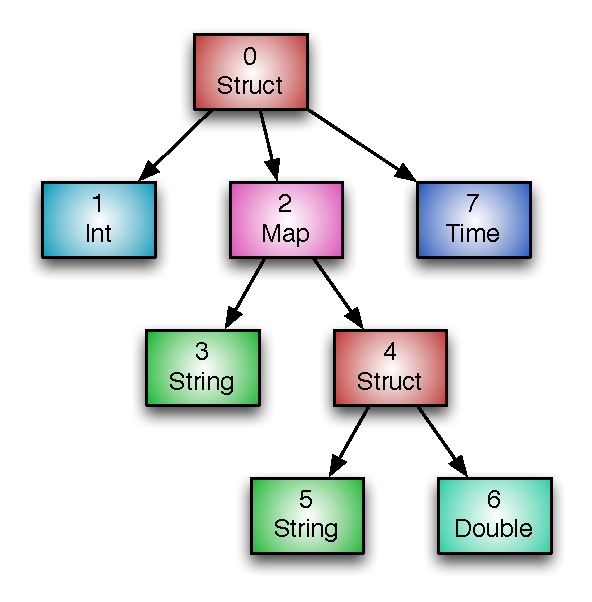
\includegraphics[width=2.4in]{TreeWriters.pdf}
  \caption{Type Tree}
  \label{type-tree}
  \vspace{-100pt}
\end{wrapfigure}

All of the rows in an ORC file must have the same schema.  Logically
the schema is expressed as a tree as in figure~\ref{type-tree}, where
the compound types have subcolumns under them.

The equivalent Hive DDL for figure~\ref{type-tree} would be:
\begin{verbatim}
create table Foobar (
  myInt int,
  myMap map<string,
            struct<myString : string,
                   myDouble: double>>,
  myTime timestamp
);
\end{verbatim}

The type tree is flattened in to a list via a pre-order traversal
where each type is assigned the next id. Clearly the root of the type
tree is always type id 0. Compound types have a field named subtypes
that contains the list of their children's type ids.

\begin{verbatim}
message Type {
  enum Kind {
    BOOLEAN = 0;
    BYTE = 1;
    SHORT = 2;
    INT = 3;
    LONG = 4;
    FLOAT = 5;
    DOUBLE = 6;
    STRING = 7;
    BINARY = 8;
    TIMESTAMP = 9;
    LIST = 10;
    MAP = 11;
    STRUCT = 12;
    UNION = 13;
    DECIMAL = 14;
    DATE = 15;
    VARCHAR = 16;
    CHAR = 17;
  }
  // the kind of this type
  required Kind kind = 1;
  // the type ids of any subcolumns for list, map, struct, or union
  repeated uint32 subtypes = 2 [packed=true];
  // the list of field names for struct
  repeated string fieldNames = 3;
  // the maximum length of the type for varchar or char
  optional uint32 maximumLength = 4;
  // the precision and scale for decimal
  optional uint32 precision = 5;
  optional uint32 scale = 6;
}
\end{verbatim}

\subsubsection{Column Statistics}

The goal of the column statistics is that for each column, the writer
records the count and depending on the type other useful fields.  For
most of the primitive types, it records the minimum and maximum
values; and for numeric types it additionally stores the sum.

\begin{verbatim}
message ColumnStatistics {
  // the number of values
  optional uint64 numberOfValues = 1;

  // At most one of these has a value for any column
  optional IntegerStatistics intStatistics = 2;
  optional DoubleStatistics doubleStatistics = 3;
  optional StringStatistics stringStatistics = 4;
  optional BucketStatistics bucketStatistics = 5;
  optional DecimalStatistics decimalStatistics = 6;
  optional DateStatistics dateStatistics = 7;
  optional BinaryStatistics binaryStatistics = 8;
  optional TimestampStatistics timestampStatistics = 9;
}
\end{verbatim}

For integer types (tinyint, smallint, int, bigint), the column
statistics includes the minimum, maximum, and sum. If the sum
overflows long at any point during the calculation, no sum is
recorded.

\begin{verbatim}
message IntegerStatistics  {
  optional sint64 minimum = 1;
  optional sint64 maximum = 2;
  optional sint64 sum = 3;
}
\end{verbatim}

For floating point types (float, double), the column statistics
include the minimum, maximum, and sum. If the sum overflows a double,
no sum is recorded.

\begin{verbatim}
message DoubleStatistics {
  optional double minimum = 1;
  optional double maximum = 2;
  optional double sum = 3;
}
\end{verbatim}

For strings, the minimum value, maximum value, and the sum of the
lengths of the values are recorded.

\begin{verbatim}
message StringStatistics {
  optional string minimum = 1;
  optional string maximum = 2;
  // sum will store the total length of all strings
  optional sint64 sum = 3;
}
\end{verbatim}

For booleans, the statistics include the count of false and true values.

\begin{verbatim}
message BucketStatistics {
  repeated uint64 count = 1 [packed=true];
}
\end{verbatim}

For decimals, the minimum, maximum, and sum are stored.

\begin{verbatim}
message DecimalStatistics {
  optional string minimum = 1;
  optional string maximum = 2;
  optional string sum = 3;
}
\end{verbatim}

Date columns record the minimum and maximum values as the number of days since
the epoch (1/1/2015).

\begin{verbatim}
message DateStatistics {
  // min,max values saved as days since epoch
  optional sint32 minimum = 1;
  optional sint32 maximum = 2;
}
\end{verbatim}

Timestamp columns record the minimum and maximum values as the number of
milliseconds since the epoch (1/1/2015).

\begin{verbatim}
message TimestampStatistics {
  // min,max values saved as milliseconds since epoch
  optional sint64 minimum = 1;
  optional sint64 maximum = 2;
}
\end{verbatim}

Binary columns store the aggregate number of bytes across all of the values.

\begin{verbatim}
message BinaryStatistics {
  // sum will store the total binary blob length
  optional sint64 sum = 1;
}
\end{verbatim}

\subsubsection{User Metadata}

The user can add arbitrary key/value pairs to an ORC file as it is
written. The contents of the keys and values are completely
application defined, but the key is a string and the value is
binary. Care should be taken by applications to make sure that their
keys are unique and in general should be prefixed with an organization
code.

\begin{verbatim}
message UserMetadataItem {
  // the user defined key
  required string name = 1;
  // the user defined binary value
  required bytes value = 2;
}
\end{verbatim}

\subsection{File Metadata}

The file Metadata section contains column statistics at the stripe
level granularity. These statistics enable input split elimination
based on the predicate push-down evaluated per a stripe.

\begin{verbatim}
message StripeStatistics {
  repeated ColumnStatistics colStats = 1;
}

message Metadata {
  repeated StripeStatistics stripeStats = 1;
}
\end{verbatim}

\section{Compression Streams}

\begin{wrapfigure}{r}{2.5in}
  \centering
  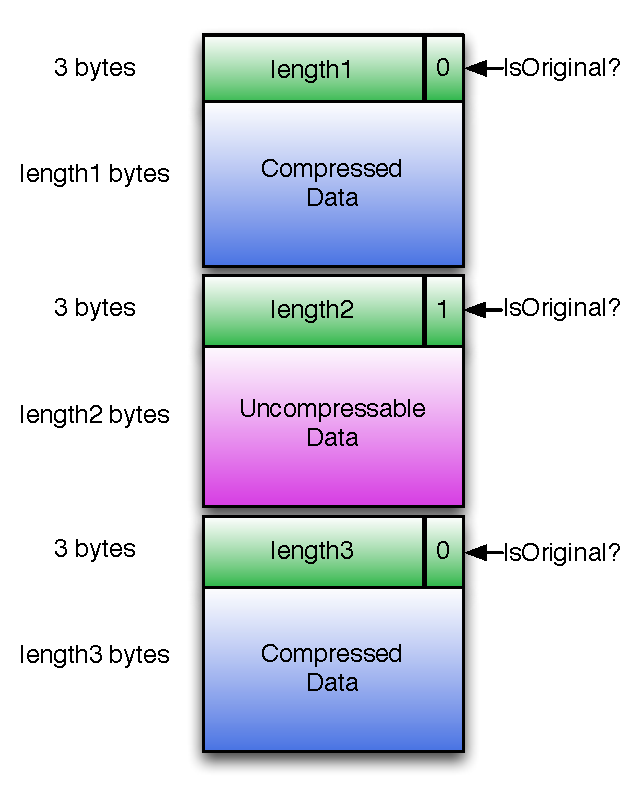
\includegraphics[width=2.4in]{CompressionStream.pdf}
  \caption{Compression Stream Structure}
  \label{compression-stream}
  \vspace{-40pt}
\end{wrapfigure}

If the ORC file writer selects a generic compression codec (zlib or
snappy), every part of the ORC file except for the Postscript is
compressed with that codec.  However, one of the requirements for ORC
is that the reader be able to skip over compressed bytes without
decompressing the entire stream. To manage this, ORC writes compressed
streams in chunks with headers as in figure~\ref{compression-stream}.
To handle uncompressable data, if the compressed data is larger than
the original, the original is stored and the isOriginal flag is
set. Each header is 3 bytes long with $ compressedLength * 2 +
isOriginal $ stored as a little endian value. For example, the header
for a chunk that compressed to 100,000 bytes would be [0x40, 0x0d,
0x03]. The header for 5 bytes that did not compress would be [0x0b,
0x00, 0x00]. Each compression chunk is compressed independently so
that as long as a decompressor starts at the top of a header, it can
start decompressing without the previous bytes.

The default compression chunk size is 256K, but writers can choose
their own value less than $2^{23}$.  Larger chunks lead to better
compression, but require more memory.  The chunk size is recorded in
the Postscript so that readers can allocate appropriately sized
buffers.

ORC files without generic compression write each stream directly
with no headers.

\section{Run Length Encoding}

\subsection{Base 128 Varint}

Variable width integer encodings take advantage of the fact that most
numbers are small and that having smaller encodings for small numbers
shrinks the overall size of the data. ORC uses the varint format from
Protocol Buffers, which writes data in little endian format using the
low 7 bits of each byte. The high bit in each byte is set if the
number continues into the next byte.

\vspace{10pt}
\begin{tabular}{| c | c |}
\hline
Unsigned Original & Serialized \\
\hline
0 & 0x00 \\
1 & 0x01 \\
127 & 0x7f \\
128 & 0x80, 0x01 \\
129 & 0x81, 0x01 \\
16383 & 0xff, 0x7f \\
16384 & 0x80, 0x80, 0x01 \\
16385 & 0x81, 0x80, 0x01 \\
\hline
\end{tabular}
\vspace{10pt}

For signed integer types, the number is converted into an unsigned
number using a zigzag encoding.  Zigzag encoding moves the sign bit to
the least significant bit using the expression $(val << 1) \wedge (val
>> 63)$ and derives its name from the fact that positive and negative
numbers alternate once encoded. The unsigned number is then serialized
as above.

\vspace{10pt}
\begin{tabular}{| c | c |}
\hline
Signed Original & Unsigned\\
\hline
0 & 0 \\
-1 & 1 \\
1 & 2 \\
-2 & 3 \\
2 & 4 \\
\hline
\end{tabular}

\subsection{Byte Run Length Encoding}
\label{byte-rle}

For byte streams, ORC uses a very light weight encoding of identical
values.

\begin{description}
\item[Run] a sequence of at least 3 identical values
\item[Literals] a sequence of non-identical values
\end{description}

The first byte of each group of values is a header than determines
whether it is a run (value between 0 to 127) or literal list (value
between -128 to -1). For runs, the control byte is the length of the
run minus the length of the minimal run (3) and the control byte for
literal lists is the negative length of the list. For example, a
hundred 0's is encoded as [0x61, 0x00] and the sequence 0x44, 0x45
would be encoded as [0xfe, 0x44, 0x45]. The next group can choose
either of the encodings.

\subsection{Boolean Run Length Encoding}

For encoding boolean types, the bits are put in the bytes from most
significant to least significant. The bytes are encoded using byte run
length encoding as described in section~\ref{byte-rle}. For example,
the byte sequence [0xff, 0x80] would be one \verb+true+ followed by
seven \verb+false+ values.

\subsection{Integer Run Length Encoding version 1}

In Hive 0.11 ORC files used Run Length Encoding version 1 (RLEv1),
which provides a lightweight compression of signed or unsigned integer
sequences. RLEv1 has two sub-encodings:

\begin{description}
\item[Run] a sequence of values that differ by a small fixed delta
\item[Literals] a sequence of varint encoded values
\end{description}

Runs start with an initial byte of 0x00 to 0x7f, which encodes the
length of the run - 3. A second byte provides the fixed delta in the
range of -128 to 127. Finally, the first value of the run is encoded
as a base 128 varint.

For example, if the sequence is 100 instances of 7 the encoding would
start with $100 - 3$, followed by a delta of 0, and a varint of 7 for
an encoding of [0x61, 0x00, 0x07]. To encode the sequence of numbers
running from 100 to 1, the first byte is $100 - 3$, the delta is -1,
and the varint is 100 for an encoding of [0x61, 0xff, 0x64].

Literals start with an initial byte of 0x80 to 0xff, which corresponds
to the negative of number of literals in the sequence. Following the
header byte, the list of N varints is encoded.  Thus, if there are
no runs, the overhead is 1 byte for each 128 integers. The first 5
prime numbers [2, 3, 4, 7, 11] would encoded as [0xfb, 0x02, 0x03,
0x04, 0x07, 0xb].

\subsection{Integer Run Length Encoding Version 2}

In Hive 0.12, ORC introduced Run Length Encoding version 2 (RLEv2),
which has improved compression and fixed bit width encodings for
faster expansion. RLEv2 uses four sub-encodings based on the data:

\begin{description}
\item[Short Repeat] used for short sequences with repeated values
\item[Direct] used for random sequences with a fixed bit width
\item[Patched Base] used for random sequences with a variable bit width
\item[Delta] used for monotonically increasing or decreasing sequences
\end{description}

\subsubsection{Short Repeat}

The short repeat encoding is used for short repeating integer
sequences with the goal of minimizing the overhead of the header. All
of the bits listed in the header are from the first byte to the last
and from most significant bit to least significant bit. If the type is
signed, the value is zigzag encoded.

\begin{itemize}
\item 1 byte header
  \begin{itemize}
  \item 2 bits for encoding type (0)
  \item 3 bits for width (W) of repeating value (1 to 8 bytes)
  \item 3 bits for repeat count (3 to 10 values)
  \end{itemize}
\item W bytes in big endian format, which is zigzag encoded if they type
  is signed
\end{itemize}

The unsigned sequence of [10000, 10000, 10000, 10000, 10000] would be
serialized with short repeat encoding (0), a width of 2 bytes (1), and
repeat count of 5 (2) as [0x0a, 0x27, 0x10].

\subsubsection{Direct}

The direct encoding is used for integer sequences whose values have a
relatively constant bit width. It encodes the values directly using a
fixed width big endian encoding.  The width of the values is encoded
using table~\ref{RleV2WidthTable}.

\begin{table}[htb]
  \begin{tabular}{| c | c | c |}
  \hline
  Width in Bits & Encoded Value & Notes\\
  \hline
  0 & 0 & for delta encoding \\
  1 & 0 & for non-delta encoding \\
  2 & 1 & \\
  4 & 3 & \\
  8 & 7 & \\
  16 & 15 & \\
  24 & 23 & \\
  32 & 27 & \\
  40 & 28 & \\
  48 & 29 & \\
  56 & 30 & \\
  64 & 31 & \\
  \hline
  3 & 2 & deprecated \\
  $5 \leq X \leq 7$ & $X - 1$ & deprecated \\
  $9 \leq X \leq 15$ & $X - 1$ & deprecated \\
  $17 \leq X \leq 21$ & $X - 1$ & deprecated \\
  26 & 24 & deprecated \\
  28 & 25 & deprecated \\
  30 & 26 & deprecated \\
  \hline
  \end{tabular}
  \caption{The 5 bit width encoding for RLEv2}
  \label{RleV2WidthTable}
\end{table}

\begin{itemize}
\item 2 bytes header
  \begin{itemize}
  \item 2 bits for encoding type (1)
  \item 5 bits for encoded width (W) of values (1 to 64 bits) using
    table~\ref{RleV2WidthTable}
  \item 9 bits for length (L) (1 to 512 values)
  \end{itemize}
\item $W * L$ bits encoded in big endian format, which is
  zigzag encoding if the type is signed
\end{itemize}

The unsigned sequence of [23713, 43806, 57005, 48879] would be
serialized with direct encoding (1), a width of 16 bits (15), and
length of 4 (3) as [0x5e, 0x03, 0x5c, 0xa1, 0xab, 0x1e, 0xde, 0xad,
  0xbe, 0xef].

\subsubsection{Patched Base}

The patched base encoding is used for integer sequences whose bit
widths varies a lot. The minimum signed value of the sequence is found
and subtracted from the other values. The bit width of those adjusted
values is analyzed and the 90 percentile of the bit width is chosen
as W.  The 10\% of values larger than W use patches from a patch list
to set the additional bits. Patches are encoded as a list of gaps in
the index values and the additional value bits.

\begin{itemize}
\item 4 bytes header
  \begin{itemize}
  \item 2 bits for encoding type (2)
  \item 5 bits for encoded width (W) of values (1 to 64 bits)
        using table~\ref{RleV2WidthTable}
  \item 9 bits for length (L) (1 to 512 values)
  \item 3 bits for base value width (BW) (1 to 8 bytes)
  \item 5 bits for patch width (PW) (1 to 64 bits)
        using table~\ref{RleV2WidthTable}
  \item 3 bits for patch gap width (PGW) (1 to 8 bits)
  \item 5 bits for patch list length (PLL) (0 to 31 patches)
  \end{itemize}
\item Base value (BW bytes) - The base value is stored as a big endian value
  with negative values marked by the most significant bit set. If it that
  bit is set, the entire value is negated.
\item Data values ($W * L$ bits) - A sequence of W bit positive values that
  are added to the base value.
\item Patch list ($PLL * (PGW + PW)$ bytes) - A list of patches for
  values that didn't fit within W bits. Each entry in the list
  consists of a gap, which is the number of elements skipped from the
  previous patch, and a patch value. Patches are applied by logically
  or'ing the data values with the relevant patch shifted W bits
  left. If a patch is 0, it was introduced to skip over more than 255
  items. The combined length of each patch (PGW + PW) must be less or
  equal to 64.
\end{itemize}

The unsigned sequence of [2030, 2000, 2020, 1000000, 2040, 2050, 2060,
  2070, 2080, 2090] has a minimum of 2000, which makes the adjusted
sequence [30, 0, 20, 998000, 40, 50, 60, 70, 80, 90]. It has an
encoding of patched base (2), a bit width of 8 (7), a length of 10
(9), a base value width of 2 bytes (1), a patch width of 12 bits (11),
patch gap width of 2 bits (1), and a patch list length of 1 (1). The
base value is 2000 and the combined result is [0x8e, 0x09, 0x2b, 0x21,
  0x07, 0xd0, 0x1e, 0x00, 0x14, 0x70, 0x28, 0x32, 0x3c, 0x46, 0x50,
  0x5a, 0xfc, 0xe8]

\subsubsection{Delta}

The Delta encoding is used for monotonically increasing or decreasing
sequences. The first two numbers in the sequence can not be identical,
because the encoding is using the sign of the first delta to determine
if the series is increasing or decreasing.

\begin{itemize}
\item 2 bytes header
  \begin{itemize}
  \item 2 bits for encoding type (3)
  \item 5 bits for encoded width (W) of deltas (0 to 64 bits)
        using table~\ref{RleV2WidthTable}
  \item 9 bits for run length (L) (1 to 512 values)
  \end{itemize}
\item Base value - encoded as (signed or unsigned) varint
\item Delta base - encoded as signed varint
\item Delta values $W * (L - 2)$ bytes - encode each delta after the first
  one. If the delta base is positive, the sequence is increasing and if it is
  negative the sequence is decreasing.
\end{itemize}

The unsigned sequence of [2, 3, 5, 7, 11, 13, 17, 19, 23, 29] would be
serialized with delta encoding (3), a width of 4 bits (3), length of
10 (9), a base of 2 (2), and first delta of 1 (2). The resulting
sequence is [0xc6, 0x09, 0x02, 0x02, 0x22, 0x42, 0x42, 0x46].

\section{Stripes}

The body of ORC files consists of a series of stripes. Stripes are
large (typically ~200MB) and independent of each other and are often
processed by different tasks. The defining characteristic for columnar
storage formats is that the data for each column is stored separately
and that reading data out of the file should be proportional to the
number of columns read.

In ORC files, each column is stored in several streams that are stored
next to each other in the file. For example, an integer column is
represented as two streams PRESENT, which uses one with a bit per
value recording if the value is non-null, and DATA, which records the
non-null values. If all of a column's values in a stripe are non-null,
the PRESENT stream is omitted from the stripe. For binary data, ORC
uses three streams PRESENT, DATA, and LENGTH, which stores the length
of each value. The details of each type will be presented in the
following subsections.

\subsection{Stripe Footer}

The stripe footer contains the encoding of each column and the
directory of the streams including their location.

\begin{verbatim}
message StripeFooter {
  // the location of each stream
  repeated Stream streams = 1;
  // the encoding of each column
  repeated ColumnEncoding columns = 2;
}
\end{verbatim}

To describe each stream, ORC stores the kind of stream, the column id,
and the stream's size in bytes. The details of what is stored in each stream
depends on the type and encoding of the column.

\begin{verbatim}
message Stream {
  enum Kind {
    // boolean stream of whether the next value is non-null
    PRESENT = 0;
    // the primary data stream
    DATA = 1;
    // the length of each value for variable length data
    LENGTH = 2;
    // the dictionary blob
    DICTIONARY\_DATA = 3;
    // deprecated prior to Hive 0.11
    // It was used to store the number of instances of each value in the
    // dictionary
    DICTIONARY_COUNT = 4;
    // a secondary data stream
    SECONDARY = 5;
    // the index for seeking to particular row groups
    ROW_INDEX = 6;
  }
  required Kind kind = 1;
  // the column id
  optional uint32 column = 2;
  // the number of bytes in the file
  optional uint64 length = 3;
}
\end{verbatim}

Depending on their type several options for encoding are possible. The
encodings are divided into direct or dictionary-based categories and
further refined as to whether they use RLE v1 or v2.

\begin{verbatim}
message ColumnEncoding {
  enum Kind {
    // the encoding is mapped directly to the stream using RLE v1
    DIRECT = 0;
    // the encoding uses a dictionary of unique values using RLE v1
    DICTIONARY = 1;
    // the encoding is direct using RLE v2
    DIRECT\_V2 = 2;
    // the encoding is dictionary-based using RLE v2
    DICTIONARY\_V2 = 3;
  }
  required Kind kind = 1;
  // for dictionary encodings, record the size of the dictionary
  optional uint32 dictionarySize = 2;
}
\end{verbatim}

\subsection{Column Encodings}

\subsubsection{SmallInt, Int, and BigInt Columns}

All of the 16, 32, and 64 bit integer column types use the same set of
potential encodings, which is basically whether they use RLE v1 or
v2. If the PRESENT stream is not included, all of the values are
present. For values that have false bits in the present stream, no
values are included in the data stream.

\vspace{10pt}
\begin{tabular}{| l | l | l | l |}
\hline
Encoding & Stream Kind & Optional & Contents \\
\hline
DIRECT & PRESENT & Yes & Boolean RLE\\
       & DATA    & No  & Signed Integer RLE v1\\
\hline
DIRECT\_V2 & PRESENT & Yes & Boolean RLE\\
          & DATA    & No  & Signed Integer RLE v2\\
\hline
\end{tabular}

\subsubsection{Float and Double Columns}

Floating point types are stored using IEEE 754 floating point bit
layout. Float columns use 4 bytes per value and double columns use 8
bytes.

\vspace{10pt}
\begin{tabular}{| l | l | l | l |}
\hline
Encoding & Stream Kind & Optional & Contents \\
\hline
DIRECT & PRESENT & Yes & Boolean RLE\\
       & DATA    & No  & IEEE 754 floating point representation\\
\hline
\end{tabular}

\subsubsection{String, Char, and VarChar Columns}

String columns are adaptively encoded based on whether the first
10,000 values are sufficiently distinct. In all of the encodings, the
PRESENT stream encodes whether the value is null.

For direct encoding the UTF-8 bytes are saved in the DATA stream and
the length of each value is written into the LENGTH stream. In direct
encoding, if the values were [``Nevada'', ``California'']; the DATA
would be ``NevadaCalifornia'' and the LENGTH would be [6, 10].

For dictionary encodings the dictionary is sorted and UTF-8 bytes of
each unique value are placed into DICTIONARY\_DATA. The length of each
item in the dictionary is put into the LENGTH stream. The DATA stream
consists of the sequence of references to the dictionary elements.

In dictionary encoding, if the values were [``Nevada'',
  ``California'', ``Nevada'', ``California'', and ``Florida'']; the
DICTIONARY\_DATA would be ``CaliforniaFloridaNevada'' and LENGTH would
be [10, 7, 6]. The DATA would be [2, 0, 2, 0, 1].

\vspace{10pt}
\begin{tabular}{| l | l | l | l |}
\hline
Encoding & Stream Kind & Optional & Contents \\
\hline
DIRECT & PRESENT & Yes & Boolean RLE\\
       & DATA    & No  & String contents\\
       & LENGTH  & No  & Unsigned Integer RLE v1\\
\hline
DICTIONARY & PRESENT          & Yes & Boolean RLE\\
           & DATA             & No  & Unsigned Integer RLE v1\\
           & DICTIONARY\_DATA & No  & String contents\\
           & LENGTH           & No  & Unsigned Integer RLE v1\\
\hline
DIRECT\_V2 & PRESENT & Yes & Boolean RLE\\
          & DATA    & No  & String contents\\
          & LENGTH  & No  & Unsigned Integer RLE v2\\
\hline
DICTIONARY\_V2 & PRESENT          & Yes & Boolean RLE\\
               & DATA             & No  & Unsigned Integer RLE v2\\
               & DICTIONARY\_DATA & No  & String contents\\
               & LENGTH           & No  & Unsigned Integer RLE v2\\
\hline
\end{tabular}

\subsubsection{Boolean Columns}

Boolean columns are rare, but have a simple encoding.

\vspace{10pt}
\begin{tabular}{| l | l | l | l |}
\hline
Encoding & Stream Kind & Optional & Contents \\
\hline
DIRECT & PRESENT & Yes & Boolean RLE\\
       & DATA    & No  & Boolean RLE\\
\hline
\end{tabular}

\subsubsection{TinyInt Columns}

TinyInt (byte) columns use byte run length encoding.

\vspace{10pt}
\begin{tabular}{| l | l | l | l |}
\hline
Encoding & Stream Kind & Optional & Contents \\
\hline
DIRECT & PRESENT & Yes & Boolean RLE\\
       & DATA    & No  & Byte RLE\\
\hline
\end{tabular}

\subsubsection{Binary Columns}

Binary data is encoded with a PRESENT stream, a DATA stream that records
the contents, and a LENGTH stream that records the number of bytes per a
value.

\vspace{10pt}
\begin{tabular}{| l | l | l | l |}
\hline
Encoding & Stream Kind & Optional & Contents \\
\hline
DIRECT & PRESENT & Yes & Boolean RLE\\
       & DATA    & No  & Binary contents\\
       & LENGTH  & No  & Unsigned Integer RLE v1\\
\hline
DIRECT\_V2 & PRESENT & Yes & Boolean RLE\\
          & DATA    & No  & Binary contents\\
          & LENGTH  & No  & Unsigned Integer RLE v2\\
\hline
\end{tabular}

\subsubsection{Decimal Columns}

Decimal was introduced in Hive 0.11 with infinite precision (the total
number of digits). In Hive 0.13, the definition was change to limit
the precision to a maximum of 38 digits, which conveniently uses 127
bits plus a sign bit. The current encoding of decimal columns stores
the integer representation of the value as an unbounded length zigzag
encoded base 128 varint. The scale is stored in the SECONDARY stream
as an unsigned integer.

\vspace{10pt}
\begin{tabular}{| l | l | l | l |}
\hline
Encoding & Stream Kind & Optional & Contents \\
\hline
DIRECT & PRESENT    & Yes & Boolean RLE\\
       & DATA       & No  & Unbounded base 128 varints\\
       & SECONDARY  & No  & Unsigned Integer RLE v1\\
\hline
DIRECT\_V2 & PRESENT   & Yes & Boolean RLE\\
          & DATA       & No  & Unbounded long base 128 varints\\
          & SECONDARY  & No  & Unsigned Integer RLE v2\\
\hline
\end{tabular}

\subsubsection{Date Columns}

Date data is encoded with a PRESENT stream, a DATA stream that records
the number of days after January 1, 1970 in UTC.

\vspace{10pt}
\begin{tabular}{| l | l | l | l |}
\hline
Encoding & Stream Kind & Optional & Contents \\
\hline
DIRECT & PRESENT & Yes & Boolean RLE\\
       & DATA    & No  & Signed Integer RLE v1\\
\hline
DIRECT\_V2 & PRESENT & Yes & Boolean RLE\\
           & DATA    & No  & Signed Integer RLE v2\\
\hline
\end{tabular}

\subsubsection{Timestamp Columns}

Timestamp records times down to nanoseconds as a PRESENT stream that
records non-null values, a DATA stream that records the number of
seconds after 1 January 2015, and a SECONDARY stream that records the
number of nanoseconds.

Because the number of nanoseconds often has a large number of trailing
zeros, the number has trailing decimal zero digits removed and the
last three bits are used to record how many zeros were removed. Thus
1000 nanoseconds would be serialized as 0x0b and 100000 would be
serialized as 0x0d.

\vspace{10pt}
\begin{tabular}{| l | l | l | l |}
\hline
Encoding & Stream Kind & Optional & Contents \\
\hline
DIRECT & PRESENT   & Yes & Boolean RLE\\
       & DATA      & No  & Signed Integer RLE v1\\
       & SECONDARY & No  & Unsigned Integer RLE v1\\
\hline
DIRECT\_V2 & PRESENT   & Yes & Boolean RLE\\
           & DATA      & No  & Signed Integer RLE v2\\
           & SECONDARY & No  & Unsigned Integer RLE v2\\
\hline
\end{tabular}

\subsubsection{Struct Columns}

Structs have no data themselves and delegate everything to their child
columns except for their PRESENT stream. They have a child column
for each of the fields.

\vspace{10pt}
\begin{tabular}{| l | l | l | l |}
\hline
Encoding & Stream Kind & Optional & Contents \\
\hline
DIRECT & PRESENT & Yes & Boolean RLE\\
\hline
\end{tabular}

\subsubsection{List Columns}

Lists are encoded as the PRESENT stream and a length stream with
number of items in each list. They have a single child column for the
element values.

\vspace{10pt}
\begin{tabular}{| l | l | l | l |}
\hline
Encoding & Stream Kind & Optional & Contents \\
\hline
DIRECT & PRESENT & Yes & Boolean RLE\\
       & LENGTH  & No  & Unsigned Integer RLE v1\\
\hline
DIRECT\_V2 & PRESENT & Yes & Boolean RLE\\
           & LENGTH  & No  & Unsigned Integer RLE v2\\
\hline
\end{tabular}

\subsubsection{Map Columns}

Maps are encoded as the PRESENT stream and a length stream with number
of items in each list. They have a child column for the key and
another child column for the value.

\vspace{10pt}
\begin{tabular}{| l | l | l | l |}
\hline
Encoding & Stream Kind & Optional & Contents \\
\hline
DIRECT & PRESENT & Yes & Boolean RLE\\
       & LENGTH  & No  & Unsigned Integer RLE v1\\
\hline
DIRECT\_V2 & PRESENT & Yes & Boolean RLE\\
           & LENGTH  & No  & Unsigned Integer RLE v2\\
\hline
\end{tabular}

\subsubsection{Union Columns}

Unions are encoded as the PRESENT stream and a tag stream that controls which
potential variant is used. They have a child column for each variant of the
union. Currently ORC union types are limited to 256 variants, which matches
the Hive type model.

\vspace{10pt}
\begin{tabular}{| l | l | l | l |}
\hline
Encoding & Stream Kind & Optional & Contents \\
\hline
DIRECT & PRESENT & Yes & Boolean RLE\\
       & DATA    & No  & Byte RLE\\
\hline
\end{tabular}

\subsection{Indexes}

The row indexes consist of a ROW\_INDEX stream for each primitive
column that has an entry for each row group. Row groups are controlled
by the writer and default to 10,000 rows. Each RowIndexEntry gives the
position of each stream for the column and the statistics for that row
group.

The index streams are placed at the front of the stripe, because in
the default case of streaming they do not need to be read. They are
only loaded when either predicate push down is being used or the
reader seeks to a particular row.

\begin{verbatim}
message RowIndexEntry {
  repeated uint64 positions = 1 [packed=true];
  optional ColumnStatistics statistics = 2;
}

message RowIndex {
  repeated RowIndexEntry entry = 1;
}
\end{verbatim}

To record positions, each stream needs a sequence of numbers. For
uncompressed streams, the position is the byte offset of the RLE run's
start location followed by the number of values that need to be
consumed from the run. In compressed streams, the first number is the
start of the compression chunk in the stream, followed by the number
of decompressed bytes that need to be consumed, and finally the number
of values consumed in the RLE.

For columns with multiple streams, the sequences of positions in each
stream are concatenated. That was an unfortunate decision on my part
that we should fix at some point, because it makes code that uses the
indexes error-prone.

Because dictionaries are accessed randomly, there is not a position to
record for the dictionary and the entire dictionary must be read even
if only part of a stripe is being read.

\end{document}
